\chapter{Background} \label{chapBackground}
\section{Application Areas}
\subsection{Forest Carbon Sequestration Prediction}
The first problem we explore in this work assessing carbon sequestration in forests. Forest are a massive sink of carbon and protecting and managing our forests is a critical tool in the fight against climate change \cite{Griscom2017NaturalSolutions}. 
It is especially important that we keep existing forests intact, because clearing them can result in substantial CO\textsubscript{2} emissions. 
One tool to incentivising this is "carbon credits," which are payments to the landowner to keep the carbon sequestered. These payments are often made by business or governments who have pledged to meet certain emission targets but cannot fulfil them immediately by reducing their CO\textsubscript{2} output. Instead, they "offset" these emissions by paying to have a commensurate amount of CO\textsubscript{2} emissions prevented. This is helpful because some activities are more challenging to de-carbonize than others. 
It is expected that demand for carbon credits will rise by a factor of 50 by 2050 according to a McKinsey report \cite{Blaufelder2021AChallenge}. 

Unfortunately, there is widespread concern that carbon credits do not actually deliver the benefits that they promise. On issue is "additionality," which reflects the concern that a credit may be issued even when the business-as-usual outcome would not have resulted in releasing the carbon \cite{Gillenwater2011TheProgramme}.
The second issue is "leakage," where sequestered carbon is later released. An example of this is forest fires releasing CO\textsubscript{2} that was claimed to be sequestered \cite{NYTimes}. These two issues deserve rigorous and multi-faceted treatment to guarantee that carbon credits actually have the intended impacts. A final consideration is much more straightforward to address: the fact that the carbon content of a forest must be accurately estimated for a credit to be meaningful. There are a variety of works showing that systematic over-crediting is common \cite{Badgley2022SystematicProgram,West2020OverstatedAmazon} due to biased modeling efforts or human errors. This is one area where technology can play a role, by improving upon simple regional models with empirical and site-specific information. 

A common method for accurately estimating the carbon content of a forest is using per-tree methods. Each tree is located and the carbon content of each one is estimated individually. The per-tree carbon content can be regressed from phenotypic values such a basal (crown) area \cite{Torres2013UsingMexico} or predicted directly from images using machine learning \cite{Reiersen2022ReforesTree:Imagery}. Our work on this topic focuses on this first stage: detecting trees.

\subsection{Forest Fire Mitigation} 
Destructive forest fires have increased dramatically over the past decades \cite{spreading_like_wildfire, ayanz2021, nfn2022}. This is due in large part to climate change, which leads to hotter and drier weather along with stronger winds \cite{spreading_like_wildfire}. This has also led to increased forest mortality from pests expanding their range, such as the mountain pine beetle in the Western US \cite{Jenkins2014AndFuels}. Humans have also contributed more directly to fires by suppressing small fires which causes fuel to build up over time. Finally, there is an increase in ignition sources from careless human activity and infrastructure such as power lines. These fires are now more dangerous to humans and property because of their scale and speed as well as increasing habitation in close proximity to forests, termed the urban-woodland interface. The ecological consequences of fire are also increasingly dire. Historical fires were a natural part of the ecosystem and the vegetation was able to regenerate due to surviving trees and un-burned seeds. The intensity of modern fires completely destroys all vegetation, making it much harder to for regions to regrow. This can lead to erosion and eventual transition from forest to grassland.

It is becoming increasingly clear that reactive firefighting is insufficient to combat fires of this magnitude and preemptive mitigation efforts are required. One way to actively reduce the risk of destructive fires is by fuel management, or removing dense understory vegetation \cite{Fire2021FuelsManagement, WildlandFireResiliencyProgram20214Plan, Agriculture2019HazardousComplex}. This is a challenging problem due to the sheer area of forested land and the limited resources currently put toward preemptive efforts \cite{spreading_like_wildfire}.

Fuel management is physically demanding and requires specialized knowledge, and this has led to increasing concerns about labor shortages \cite{CommisionGlobalDivision}. 
The threat of forest fires has driven increasing government interest in technological innovation, with the USDA \cite{USDA2023USDAGrant} and NASA \cite{SPSO2023Research2023} providing funding in this area. This grant opportunities address the need for pre-fire understanding and mitigation efforts rather than only reactive measures.
A recent robotics project proposed a multi-robot team that could autonomously remove vegetation \cite{couceiro2019semfire}. In this work, an unmanned ground vehicle can traverse the environment and mechanically grind vegetation, rendering it a much less potent fuel source. This robot only has an understanding of its local environment, so the proposed concept relies on drones to map the environment beforehand. These drones much determine both the geometric structure of the scene, so the robot can avoid obstacles, and the locations of fuel, so the robot can determine where to go. Our work tackles this fuel mapping problem from the drone, and also proposes to extend this work to broader regions by also predicting vegetation locations from remote sensing data. 


\section{Sources of Data for Forestry}
Making intelligent forestry decisions requires digital data \cite{digitalForestry2009} and the previous section highlights two examples where this is critical. Unfortunately, it is challenging to obtain information that is both accurate and at a large enough scale to be truly useful. In this work we look at three sources of data that can inform forest management: observations from manual field work, images from small uncrewed aerial systems (sUAS or "drones"), and optical remote sensing data taken from aircraft or satellites. These three sources of data represent a trade-space between high interpretability from manual observations and high scalability from remote sensing.

\subsection{Manual Plot Measurements}
Understanding forests is still a largely manual process where foresters go into the field and measure various quantities such as tree height, diameter, density, species. In commercial contexts this is often called timber cruises \cite{ServiceFSHHANDBOOK} and in ecology it is often called forest inventories \cite{USForestServiceDepartmentofAgriculture2016FORESTPLOTS}. Since this process is laborious, the established practice is to only take measurements at points or plots distributed throughout the environment \cite{Town2018ForestryMethods}. Choosing how to balance the size versus number of plots and where to take samples requires substantial  domain expertise to achieve accurate and unbiased estimates of for the whole region.

\subsection{Drone Surveys}
Drones equipped with cameras are becoming increasingly popular in forestry \cite{CristanDronesManagement,Tang2015DronePractices}. This is driven by their comparatively low cost, easy of use, and flexibility. As described by \cite{Tang2015DronePractices}, drones fill a crucial operational gap by capturing higher resolution data than crewed aircraft or satellites. This has allowed motivated their use for a wide variety of forestry tasks that require granular information.

Cameras are a commonly-used sensor on drones because of their low cost and weight. Drones are often equipped with a commodity-grade GPS for navigation, which means that the captured images can be tagged with a approximate absolute location. Even though drones can be flown manually, it is common in forestry applications to use software such as QGronndControl or DroneDeploy \cite{} to plan an autonomous flight pattern. The user defines a perimeter of the area and sets parameters such as the survey pattern, altitude, and image density. The area that a drone can cover varies by a based on the drone and these parameters, but it is often on the order of several acres. Similarly, the spatial resolution of the data varies, but is on the order of centimeters per pixel.  While drones are a powerful tool, the raw data from them must generally be processed in a domain-specific manner to obtain the ecological information that is required by the end user.  

\subsection{Remote Sensing}
Remote sensing data is captured by sensors onboard satellites or airplanes and is rapidly becoming a critical tool for environmental monitoring \cite{Parra2022RemoteMonitoring}. This is largely because these sensors observe large---potentially global---regions and this data is often available freely to the public. 
Remote sensing data can be from many modalities, such as light detection and ranging (LiDAR) \cite{LiDARForestryBeland2019}, synthetic aperture radar (SAR) \cite{Hall2020WhatEarthdata}, and electro-optical (EO) data.
In this work we focus on electro-optical data, since it is prevalent and easy to interpret. This data is conceptually very similar to images taken by a traditional camera. However, while most terrestrial cameras only capture red-green-blue (RGB) information, remote sensing instruments often capture more distinct spectral bands, termed multi- or hyper-spectral data. Another consideration is that the information is often provided in a processesed form, where various corrections have been applied, such as removing atmospheric effects, stitching images together, and resampling the data to lie on an axis aligned, e.g. East-North, grid. 
Optical remote sensing data has been used for numerous forestry applications such as mapping forest coverage \cite{ Hansen2013High-resolutionChange} and mapping forest type \cite{Kempeneers2011DataMapping}. These characteristics are automatically interpreted from the various spectral bands captured by the satellite and this often requires domain- and sensor-specific modeling. Furthermore, a common issue with this work is the low spatial resolution of the result. For example, the forest extent mapping conducted by Hansen et. al. \cite{Hansen2013High-resolutionChange} was only available at 30 meter resolution, because that was the resolution of the input data from the LandSat satellite.

%{Ewald2023Remote}. One common issue


\section{Interpreting Forestry Data}
As discussed in the previous section, there are 
\subsection{Understanding the Geometry of Scenes}
\subsubsection{Structure from Motion}
In general, commodity drones produce only monocular images with potentially a low-accuracy GPS and orientation estimate. A common approach for estimating geometric from this type of data is photogrametry, also known as structure from motion or 3D reconstruction.  Preliminary reconstructions of realistic large-scale scenes began with academic work such as \cite{Agarwal2009}. Over the last decade, numerous commercial and open sources software have been developed for this task, such as Agisoft Metashape \cite{AgisoftMetashape} and COLMAP \cite{schoenberger2016mvs, schoenberger2016sfm}, respectively.

The details vary by application and assumption, but a common pipeline is the following. First, distinctive features are detected in each image. These represent small patches of pixels which are likely to be distinctive, such as corners and edges. Then, features are matched between images, based on the local appearance. 
Given these correspondences, multiple quantities can be estimated. The first is the location of these matched points in the 3D space, using triangulation between the cameras. The second is the location of the cameras. Finally, if the camera isn't accurately calibrated, it's common to estimate the parameters which describe how points in the world appear on the image. Given the interplay between all of these elements, it's critical to estimated them together in a global joint optimization. The class of techniques for solving this problem are termed bundle adjustment \cite{Triggs2000BundleSynthesis}. After the locations of the cameras have been estimated, it is possible to construct a dense pointcloud or mesh representation of the scene, an example of which can be seen in Figure \ref{fig:background:camera_locations}.

Photogrametry has been used in a variety of recent works on understanding forests \cite{Swayze2021InfluenceDensity, doi:10.1139/cjfr-2020-0433}. A notable work in this space is that of Young et. al. \cite{Young2022}. This work studies impacts of different drone fight patterns and Metashape processing parameters on the quality of tree detection in complex coniferous forests. They use extensive experiments to propose a flight pattern and set of parameters that can be used in other tree detection applications.
\begin{figure}
    \centering
    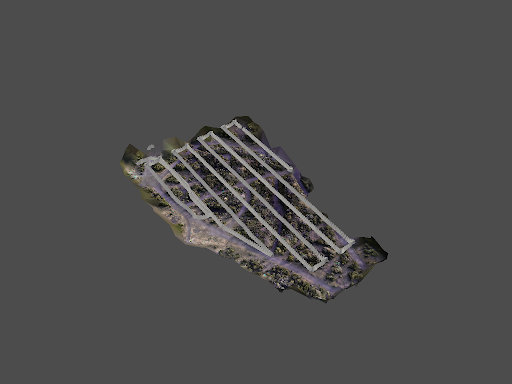
\includegraphics[width=0.8\textwidth, trim={4cm 3cm 4cm 4cm}, clip]{figs/methods/structure_from_motion/camera estimation.png}
    \caption{An example 3D reconstruction with the camera locations from the drone survey visualized.}
    \label{fig:background:camera_locations}
\end{figure}

%These solvers are becoming increasingly robust, and are well-suited to reconstructing scenes captured by drone surveys because the same location is often seen across many images.

\subsubsection{Simultaneous Localization and Mapping (SLAM)}
Structure from motion is a powerful tool, but a key limitation is that it can only be used to map the environment after a mission is complete. In settings where a drone is operating autonomously in complex environment such as under the canopy, it is important that it understands where it is in relation to obstacles in real time. This problem is challenging because it requires completing two challenging tasks at once: building a map of the world while estimating where the robot is within the map. This problem is known in the robotics literature as simultaneous localization and mapping (SLAM) \cite{durrant2006simultaneous}. This refers to the fact that in a new environment, the robot must build a map of the world at the same time as figuring out where it is in this map. 

A variety of generic SLAM approaches have been proposed in recent years, such as LIO-SAM \cite{}, VIL-SLAM \cite{}, and LOAM \cite{}. These approaches are often primarily tested in urban or indoors environments and the work of Garforth et. al. \cite{Garforth2019VisualSLAM} explains some of the attributes that make forests difficult environments for vision-based SLAM. One work that proposes a forest-specific SLAM approach is SLOAM \cite{Chen2020SLOAM:Inventory}. This approach detects tree trunks and uses them as landmarks to increase the localization accuracy and robustness.

\subsection{Understanding the Content of Images}
Given the increasing amount of raw data about our forests, a key question is how to extract meaningful insights. Quantities such as the extent, species composition, health, or biomass of a forest can be more easily used to make management decisions. Automated processing methods can free domain experts from the laborious task of interpreting this data by hand. There has been a steady shift from methods which are hand-designed to those which use supervised machine learning. This means fitting some sort of model to existing data that shows the input information and the correct interpretation. Then this model can be used to generate predictions on new data. Over the last decade there have been an explosion of approaches relying on deep learning \cite{Lecun2015DeepLearning}, which is a subset of machine learning using models that have multiple hiararchical processing steps. This requires dramatically more parameters than previous machine learning models but allows greater flexibility and expressivity. This means that less human intuition is required but also means that large quantities of labeled data are expected to achieve good performance. 
\subsubsection{Semantic Segmentation}
Semantic segmentation is the task of assigning a classification label to every pixel in an image. In the forestry domain, these classes could be broad, such as trees, shrubs, and grasses or more granular, such as different species of trees. An example image can be seen in Figure \ref{fig:background:semantic_seg_example}.

\begin{figure}
    \centering
    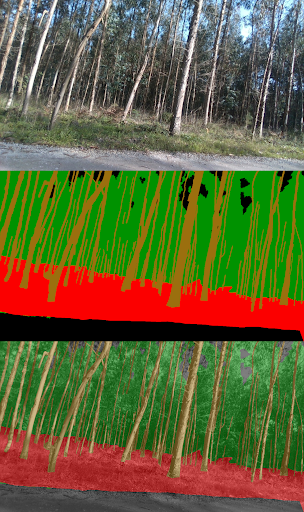
\includegraphics[width=0.45\textwidth, trim={0 340px 0 0}, clip]{figs/background/automated_understanding/segmentation_example.png}
    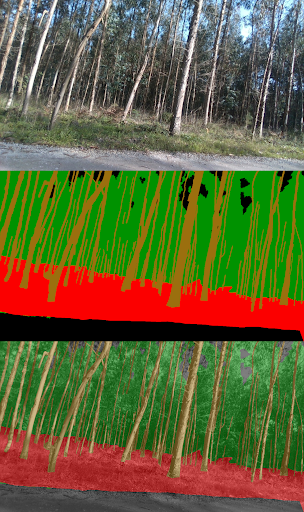
\includegraphics[width=0.45\textwidth, trim={0 170 0 170}, clip]{figs/background/automated_understanding/segmentation_example.png}
    \caption{A visualization of the goal of semantic segmentation. The input image is on the left, and the desired output is on the right, color-coded by class. Red is understory fuel, green is canopy, brown is trunk, and black is background such as bare earth and sky}
    \label{fig:background:semantic_seg_example}
\end{figure}

An early work on semantic segmentation with deep learning was Fully Convolutional Network \cite{Shelhamer2017FullySegmentation} which took early insights from image classification and adapted them to give per-pixel class predictions. Shortly following this was U-Net \cite{RonnebergerUNET2015}, which had an encoder-decoder architecture with skip connections to preserve high-resolution details. A wide variety of approaches have been developed since then using slight variations on these initial concepts. A recent shift has been toward using transformers \cite{Vaswani2017AttentionNeed} which has resulted in work such as Segformer \cite{Xie2021} and SegNext \cite{Guo2022SegNeXt:Segmentation}.

A significant fraction of semantic segmentation works were evaluated on datasets related to autonomous vehicles, sch as CityScapes \cite{Cordts2016}. However, these methods have been shown to be applicable to other domains, and recent work has explored them in the context of drone forestry images \cite{Nogueira2017SemanticConvNets, Neves2020SemanticU-net}. 

\subsubsection{Object Detection}
